\documentclass[12pt]{article}
\usepackage[english]{babel}
\usepackage[utf8x]{inputenc}
\usepackage[T1]{fontenc}
\usepackage{scribe}
\usepackage{listings}
\usepackage{graphics, graphicx}
\usepackage{enumerate}
\usepackage{enumitem}
\usepackage{tcolorbox}
\usepackage{adjustbox}
\usepackage{mathtools}
\usepackage{amsmath}
\usepackage[edges]{forest}
\usepackage{multicol}
\usepackage{bbm}
\setlength{\columnsep}{1cm}
\DeclarePairedDelimiter{\ceil}{\lceil}{\rceil}

\newcommand{\forceindent}{\leavevmode{\parindent=1.3em\indent}}
\newcommand{\dbt}{\forceindent \forceindent}
\graphicspath{ {./images/} }

\CourseName{Comtemporary Algorithms T.II/2019-20}
\Scribe{Kanokpon \& Kanokpon}
\Lecturer{Dr. Kanat Tangwongsan}
\LectureNumber{18}
\LectureDate{15 January 2020}
\LectureTitle{Random walks for Network Analysis I}

\lstset{style=mystyle}

\newlist{steps}{enumerate}{1}
\setlist[steps, 1]{label = Step \arabic*:}

\begin{document}
\MakeScribeTop
\section{Random Walk on graph}
Start at initial vtx. Pick neighbor at random and visit there. Then we measure the probability distribution of the random walk.
\begin{center}
	\begin{tikzpicture}[scale=0.2]
	\tikzstyle{every node}+=[inner sep=0pt]
	\draw [black] (11,-34.8) circle (3);
	\draw (11,-34.8) node {$a$};
	\draw [black] (58.6,-34.8) circle (3);
	\draw (58.6,-34.8) node {$d$};
	\draw [black] (37.5,-22.7) circle (3);
	\draw (37.5,-22.7) node {$e$};
	\draw [black] (36.9,-34.8) circle (3);
	\draw (36.9,-34.8) node {$c$};
	\draw [black] (31.6,-51.6) circle (3);
	\draw (31.6,-51.6) node {$b$};
	\draw [black] (11.724,-31.891) arc (162.46841:17.53159:24.2);
	\draw [black] (28.605,-51.695) arc (-92.81119:-165.58563:18.592);
	\draw [black] (57.644,-37.641) arc (-22.29329:-93.92512:23.219);
	\draw [black] (14,-34.8) -- (33.9,-34.8);
	\draw [black] (39.9,-34.8) -- (55.6,-34.8);
	\draw [black] (13.73,-33.55) -- (34.77,-23.95);
	\draw [black] (40.1,-24.19) -- (56,-33.31);
	\draw [black] (36,-37.66) -- (32.5,-48.74);
	\end{tikzpicture}
\end{center}

\begin{itemize}
	\item start at initial vtx.
	\item Follow an edge uniformly at random
\end{itemize}

\begin{center}
	probability of visiting each vertex\\
	\begin{tabular}{|c| c| c| c| c| c|} 
		\hline
		& a & b & c & d & e \\ [0.5ex] 
		\hline\hline
		$\vec{P}_0$ & 1 & 0 & 0 &0 &0 \\ 
		\hline
		$\vec{P}_1$ & 0 & $\frac{1}{4}$ & $\frac{1}{4}$ & $\frac{1}{4}$ & $\frac{1}{4}$ \\
		\hline
		$\vec{P}_2$ &  $\vec{P}_2(a) $&  & & & \\ [1ex] 
		\hline
	\end{tabular}
\end{center}

$\vec{P}_2(a) = \frac{1}{3}\vec{P}_1(b) + \frac{1}{3}\vec{P}_1(c) + \frac{1}{4}\vec{P}_1(d)$\\

$\vec{P} \in \mathbb{R}^n$ $\vec{P} \geq 0$\\

$\mathbbm{1}^T \vec{P} \sum_{u \in v} \vec{P}(u)\cdot 1$\\

$P_{t+1}(u) = \sum_{v~u} \frac{1}{dv}P_t(v)|\vec{P}_{t+1}=\underbrace{AD^{-1}}_{\text{walk matrix}}\vec{P}_t$

\section{Lazy walk}
\begin{itemize}
	\item w.p. $\frac{1}{2}$ : stay put
	\item w.p. $\frac{1}{2}$ : pick a random neighbor
\end{itemize}
$$P_{t+1} (u) = \frac{1}{2}P_t(u)+\frac{1}{2}\sum_{v~u}\frac{1}{dv}P_t(v)$$
\begin{eqnarray*}
 \underbrace{ \left(\begin{matrix}
  	\frac{1}{d_1} &  & &\\
  	&\frac{1}{d_2}  & &\\
  	& &\ddots &\\
  	&&&\frac{1}{d_n}
  \end{matrix}\right)}_{\left(\begin{matrix}
  {d_1} &  & &\\
  &{d_2}  & &\\
  & &\ddots &\\
  &&&{d_n}
\end{matrix}\right)^{-1}}
	\left(\begin{matrix}
		P(1)\\
		\vdots\\
		P(n)\\
	\end{matrix}\right)
	=\left(\begin{matrix}
		\frac{P(1)}{d(1)}\\
		\vdots\\
		\frac{Pn}{d(n)}\\
	\end{matrix}\right)
\end{eqnarray*}
$$\vec{P}_{t+1} = \frac{1}{2}I\vec{P}_t + \frac{1}{2}AD^{-1}\vec{P}_t=\frac{1}{2}(I+AD^{-1})\vec{P}_t$$
\subsection{Steady-state distribution}
There is a steady-state distribution appears at each vertex with probability propotional to its degree.
$$\pi(u) = \frac{d(u)}{\sum_{v\in V}d(v)}$$
\begin{eqnarray*}
	\text{WTS. } \Pi &=& W\Pi\\
	&\cdots& w \cdot w\cdot w\cdot w\vec{P}_o\\
	\Pi &=& \lim _{t \to \infty} w^t \vec{P}_o\\
	\Pi &=& W \cdot \Pi
\end{eqnarray*}
\begin{lemma} When the steady-state dist. exists, $\Pi$ is uniquely $\Pi(u)=\frac{du}{\sum dv}=\frac{du}{2m}$
\end{lemma}
\begin{proof}
	\begin{align*}
	w\left(\begin{matrix}
		d_1\\
		d_2\\
		\vdots\\
		d_n\\
	\end{matrix}\right)
	&=\left(\begin{matrix}
	d_1\\
	d_2\\
	\vdots\\
	d_n\\
	\end{matrix}\right)
	 &-\text{WTS}\\
	AD^{-1}\left(\begin{matrix}
	d_1\\
	d_2\\
	\vdots\\
	d_n\\
	\end{matrix}\right)
	&=A\vec{\mathbbm{1}}
	&\vec{\mathbbm{1}} =  \left(\begin{matrix}
	\frac{1}{d_1} &  & &\\
	&\frac{1}{d_2}  & &\\
	& &\ddots &\\
	&&&\frac{1}{d_n}
	\end{matrix}\right)
	\left(\begin{matrix}
	d_1\\
	d_2\\
	\vdots\\
	d_n\\
	\end{matrix}\right)\\
	&=\begin{bmatrix}
	d_1\\
	d_2\\
	\vdots\\
	d_n\\
	\end{bmatrix} = d
	\end{align*}
\end{proof}
\textbf{Question:} How big does $t$ have to be so that $||w^t\vec{p}_0-\Pi||_2 < \varepsilon$
\subsection{Other Quantities of Interest}
\begin{align*}
\text{Hitting time } :H_{u,v} &= \mathbb{E}[T_{\text{to reach } v}|\text{start = }u]\\
\text{Comute Time }: d_{u,v}& = \mathbb{E}[T \text{to go from } u\to v \to u]\\
\text{Linearity of expectation }: c_{u,v} &= H_{uv} + H_{vu}\\
\text{Cover time from }u: C_u&=\mathbb{E}[\text{have visited all vtxes of $G$ start at $u$}]\\
\text{Cover time of G }: C_G &= \max_u C_u
\end{align*}
\section{Random walks}
\begin{theorem}[]
	$\text{Let } G = (V, E) \text{be a simple, connected, undirected graph. }\\
	\text{Then }C_G \geq 2m(n-1)\\$
\end{theorem}
\begin{theorem}[]
	For a connected graph $G$, if\\
	$u \neq v \in V,$ then\\
	$$C_{uv} = H_{uv} + H_{vu} = 2m R_{eff} (u~v)$$
\end{theorem}
\begin{proof}
	Thm3.1:
	\begin{align*}
	\text{$G$ is connected} &\Rightarrow G \text{ has a spanning tree $T$}\\
	C_G &\leq \sum_{\{x,y\} \in E(T)} C_{xy} &\text{[look at the Euler tour on $T$]}\\
	& \leq (n-1)2m \\
	C_{xy} &= 2m\underbrace{R_{eff}(x~y)}_{\leq R_{x~y} = 1} \leq 2m\\
	\end{align*}
\end{proof}
\begin{center}
\fbox{$H_{u \to v}1+\frac{1}{d_u}\sum_{w\sim u}H_{w \to v}$}\\
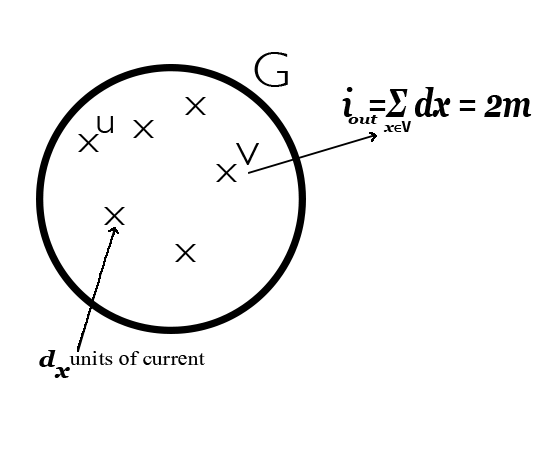
\includegraphics{Gcirc.png}
\end{center}
We can relate random walks to an electrical networks( imagine graph as a circuit with resistor on every edge).

If we create potential difference at two vertices, thus we induce an electrical flow in the graph.
\begin{eqnarray*}
	\text{potential between } u,v &=&\phi_{u,v} \in \mathbb{R}\\
	V = IR &\Longleftrightarrow& I = \frac{V}{R}\\
	&& \phi \mathbb{R}^n \to \mathbb{R}\\
	&& \phi(n) = \text{the potential of } u\\\\
	d_u &=& \sum_{w\sim u} i_{u \to w}\\
	&=& \frac{\phi(w) - \phi{u}}{R_{w\sim u}}\\
	&=& \phi(w) - \phi(u)\\
	&=& ([\phi(w) - \phi(v) ] + [\phi(v) - \phi(u) ])\\
	\frac{1}{d_u} \fbox{$d_u = [\phi(v) - \phi(u) ]d_u - [\phi(v) - \phi(w) ]$}\\
	1 &=& \underbrace{(\phi(v) - \phi(u) )}_{H_{u \to v}} - \frac{1}{d_u} \sum_{w\sim u} \underbrace{[\phi(v) - \phi(w)]}_{H_{w \to v}}\\
	H_{u\to v} &=& 1+ \frac{1}{d_u}H_{w\to v}
\end{eqnarray*}
Fix $u$ \& $v$\\

\begin{proof}
	Thm3.2:
	
	Set up four electrical networks corresponding to graph $G$
\begin{enumerate}[label=(\Alph*)]
	\item Inject $d_x$ into every vtx $x \in v$ \& take out 2$m$ from $v$
	\item Inject $d_x$ into every vtx $x \in v$ \& take out 2$m$ from $u$
	\item Inject 2$m$ into $u$ \& take out $d_x$ from every $x\in v$
	\item Inject 2$m$ into $u$ \& take out $2m$ from $v$
\end{enumerate}
\begin{itemize}
	\item claim $H_{u \to v} = \begin{matrix}(A)\\\phi(v)\end{matrix} - \begin{matrix}(A)\\\phi(u)\end{matrix}$
	\item claim $H_{v \to u} = \begin{matrix}(C)\\\phi(v)\end{matrix} - \begin{matrix}(C)\\\phi(w)\end{matrix}$
	\item claim $H_{v \to u} = \begin{matrix}(B)\\\phi(u)\end{matrix} - \begin{matrix}(B)\\\phi(v)\end{matrix}$
	\item claim $D = A+C$
\end{itemize}
\begin{align*}
	\begin{matrix}(D)\\\phi(v)\end{matrix} - \begin{matrix}(D)\\\phi(u)\end{matrix}\\
		IR_{eff(u~v)} &=\underbrace{[\begin{matrix}(A)\\\phi(v)\end{matrix} - \begin{matrix}(A)\\\phi(u)\end{matrix}]}_{H_{u \to v}} + \underbrace{[\begin{matrix}(C)\\\phi(v)\end{matrix} - \begin{matrix}(C)\\\phi(w)\end{matrix}]}_{H_{v \to u}}\\
	&=C_{uv}\\
\end{align*}
\end{proof}
\end{document}
